\label{A_FCOORDS}

Im Anschluss an die Versuche und die Berechnungen der theoretischen und realen Farbspektren sollen diese von den Teilnehmenden nun miteinander verglichen werden. Hiermit wird der Bezug zwischen den aus den Messwerten berechneten theroetisch möglichen und dem realen Farbbereich hergestellt. Der real gemessene und der berechnete Farbbereich sind in Abbildung \ref{A_Farbdreieck} dargestellt.

\begin{figure}[h]
	\centering
	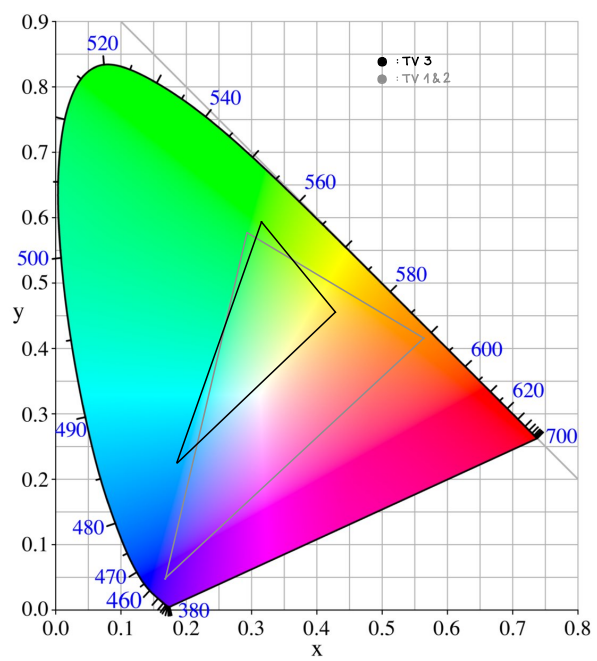
\includegraphics[scale=0.6]{Images/A_Farbdreieck.png}
	\caption{Berechneter und gemessener Farbraum des Beamers}
	\label{A_Farbdreieck}
\end{figure}

Sehr deutlich zu erkennen ist, dass der Farbraum des realen Beamers weitaus kleiner ist im Vergleich zum berechneten Erwartungswert. Der Anteil des grünen Lichtes (approximativ die y-Koordinate) des Lichtes ist auch bei voller Ansteuerung von Rot bzw. Blau immer höher in den Realwerten im Vergleich zu den in \ref{sec:Erwartungswerte} berechneten Erwartungswerten, lediglich der Grünkanal selbst ist bei Real- und Erwartungswerten nahezu gleich. Der reale Farbbereich überschneidet sich nur noch zu 19\% mit dem Adobe-Farbraum, bzw. zu 27\% mit dem sRGB-Farbraum, wenn mit der gleichen Methode der Flächeninhaltsberechnung wie in \ref{sec:Erwartungswerte} gearbeitet wird.

Begründet werden kann diese Verschlechterung durch eine Alterung der LCD-Elemente. Auch ohne Messungen konnten die Teilnehmer ein sehr grünliches Bild auch bei blauen und roten Bildern beobachten, d.h. die Rot- und Blaupunkte wurden stark beeinträchtigt. Zusätzlich wurden die Verluste an den dichroitischen Spiegeln nicht betrachtet, welche evtl. ein anderes Reflektionsspektrum als angenommen besitzen. Dies gilt auch für den Rekombinationsspiegel, welcher zusätzliche Verluste einbringt, und nicht berücksichtigt wurde. Auch sind Verluste an den LCD-Elementen selbst nicht betrachtet worden. All diese Verluste erklären gut die Abweichungen zwischen Real- und Erwartungswert, können hier jedoch nicht quantifiziert werden.

\subsubsection{Fazit}

In diesem Versuch konnten erfolgreich einige der Elemente eines handelsüblichen LCD-Beamers bemessen werden. Eine Berechnung des theoretisch möglichen Farbraumes war möglich, und lieferte plausible Werte. Die geringe Übereinstimmung mit dem realen Farbraum konnte ebenso erklärt werden durch eine Alterung des Beamers. Den Studierenden wurde somit ein Einblick in einige der wichtigen Elemente eines solchen Beamers geliefert, während weiter Fragestellungen wie z.B. der Einfluss der LCD-Schirme oder des Rekombinationsspiegels zu einer tieferen Auseinandersetzung mit dem Material geführt haben.